%!TEX TS-program = xelatex
%!TEX root = ../../maxwell2018thesis.tex

\chapter[Information Retrieval]{Information Retrieval:\\A History and Background}\label{chap:ir_background}
It may be fair to say that \emph{searching for information} is now a commonplace activity within our daily lives. Given the familiarity and near ubiquity of the search box (as shown below) on contemporary human-computer interfaces, one may be forgiven into na\"{i}vely thinking that research and development into the underlying \emph{search engine} that one interacts with when using the search box was focused exclusively upon the domain of \emph{web search}, where names like \emph{Google}, \emph{Bing} and \emph{AltaVista}\footnote{This name might spring to mind for those with more of a historical knowledge of search engines. The author of this thesis has very vague memories using AltaVista when he was around eight years old\dots} spring to mind. Despite potential negatives that these technologies may bring -- turning us into so-called \emph{shallow thinkers}~\citep{carr2008google_stupid}, for example -- search engines today by and large make our lives easier, allowing us to find that proverbial needle in the haystack with relative ease.

\begin{figure}[h]
    \centering
    \vspace{4mm}
    \resizebox{1\hsize}{!}{
    
\includegraphics{figures/ch2-searchbox.pdf}}
    \label{fig:searchbox}
    \vspace{-5mm}
\end{figure}

The research and development that has gone into search and indexing technologies that allow us to find that proverbial needle has been going on for decades, long before the advent of computers and associated communication technologies, such as the~\gls{acr:www}. This research has led to the formation of the study of~\gls{acr:ir} and the development of contemporary~\gls{acr:ir} systems.\footnote{Some within the~\gls{acr:ir} may consider this to be a contentious point: does the~\gls{acr:ir} community embrace those wishing to contribute? One of the most famous research papers associated with~\gls{acr:ir} discussing Google's \emph{PageRank} algorithm~\citep{page1998pagerank}, was rejected from SIGIR. See \url{http://rakaposhi.eas.asu.edu/f08-cse494-mailarchive/msg00037.html} (last accessed March 6\textsuperscript{th}, 2018) for more information.} With this field of study has come with it the development a \emph{de facto} approach to conducting~\gls{acr:ir} research, along with various retrieval models and means with which to evaluate their effectiveness. It is in this vain that we frame this chapter: beginning with a brief history of~\gls{acr:ir} research (Section~\ref{sec:ir_background:history}), we then consider the basic assumptions and approaches used within the field for experimental research (Section~\ref{sec:ir_background:basics}) and how we evaluate these experiments (Section~\ref{sec:ir_background:evaluation}).

\section{A (Brief) History of Information Retrieval}\label{sec:ir_background:history}
It has only been over the last two decades that search engines have become commonplace in our daily lives, primarily for the domain of web search -- as discussed in Section~\ref{sec:ir_background:history:www}. Contemporary search technologies are essentially ubiquitous, integrating seamlessly with computer operating systems (as illustrated in Figure~\ref{fig:search_integration}). Computerised~\gls{acr:ir} systems have however existed as far back as the late 1940's (as demonstrated by~\citealp{holmstrom1948univac}), with more primitive approaches (both mechanised and manual categorisation approaches) to sorting and categorising information being developed even earlier.

\begin{figure}[t!]
    \centering
    \resizebox{1\hsize}{!}{
    
\includegraphics{figures/ch2-search_integration.png}}
    \caption[Search Integration within Windows\textregistered~10]{An example of search integration within the Windows\textregistered~10 operating system. Here, results for the query \texttt{glasgow university} are shown. Results are returned from the \emph{Bing} search engine; one can also search for files on their local computer.}
    \label{fig:search_integration}
\end{figure}

\subsection{Libraries and Mechanisation}
Before the advent of computers and technologies such as the~\gls{acr:www}, one of the first locations in which one would consult when looking for information would be a \emph{library}. Containing a large volume of books discussing a virtually unlimited range of categories, the need for providing a means to organise (and thus locate) information with relative ease was of paramount importance. \emph{Catalogues} provide such a way in which to do this, with ancient Greek poet Callimachus being the first person to create such an item, in the third century BC~\citep{eliot2009companion}. A more recognisable approach to categorising content was devised by~\cite{dewey1891dcs} with the \emph{Dewey Decimal System}. The use of cards as an \emph{indexing system} was also considered by individuals such as~\cite{soper1920patent} who invented a system of providing information on what category a card belonged to based upon a punched hole.

In order to speed up the process of finding useful material, mechanisation was also extensively used. Allowing for searching at the rate of 600 cards per minute, Luhn devised in the early 1950's a mechanised system which utilised punchcards and light. As stated by~\cite{sanderson2012history_of_ir}, this was also around the time that the term~\glsfirst{acr:ir} was used~\citep{mooers1950theory}. It was at this point that computer technology was rapidly developing as a base for a viable, faster alternative to manual and mechanised approaches. This therefore led to the demise of mechanised systems, as highlighted by~\cite{jahoda1961electronic_searching}.

\subsection{The Rise of Computers}
Computers today provide the medium with which we closely associate a typical~\gls{acr:ir} system.~\cite{sanderson2012history_of_ir} state that digital storage capacity (e.g. hard disks) roughly doubles every two years -- similar to the famous \emph{Moore's Law}~\citep{moore1965law}, which observes that the number of transistors in a processor (or integrated circuit) doubles roughly every two years. Indeed, the speed at which contemporary computers can search vast indexes and databases of content is vastly superior to traditional cataloguing approaches.

One of the earliest discussions about the use of computers as the basis for an~\gls{acr:ir} system specifically mentioned the~\gls{acr:univac}.~\cite{holmstrom1948univac} described a (potentially pre-production)~\gls{acr:univac} system that was capable of searching for text with a given \emph{reference code} stored on steel tape.~\cite{mitchell1953univac_million} also showed a~\gls{acr:univac} system capable of searching one million records indexed by six subject codes. It was around this time that computers began to replace the traditional librarian, being able to provide a much more effective and cost effective means of trawling through a library's records.

From this point on, work began to establish~\gls{acr:ir} as a scientific field. Gerard Salton established a large~\gls{acr:ir} research group, initially at Harvard University. Many of the basic constructs which we utilise within~\gls{acr:ir} today were established around this time, in addition to the experiments undertaken by~\cite{cleverdon1962cranfield_experiments} -- known as the \emph{Cranfield Experiments}. These experiments established the concept of using words to index documents within an~\gls{acr:ir} system, providing advancements in indexing technology.~\cite{luhn1957ranking_query} proposed, and~\cite{maron1959probabilistic_indexing} tested, an approach to ranking that scored documents in a collection in relation to a user issued \emph{query} -- a concept that is central to contemporary~\gls{acr:ir} systems. A detailed explanation of these concepts are provided later in this chapter -- refer to Section~\ref{sec:ir_background:basics}.

\begin{figure}[t!]
    \centering
    \resizebox{1\hsize}{!}{
    
\includegraphics{figures/ch2-yahoo.png}}
    \caption[Screenshot of \emph{Yahoo!} Search, July 1998]{A screenshot of the landing page of \emph{Yahoo!}, as shown on July 5\textsuperscript{th}, 1998. Notice the link for the 1998 \emph{FIFA World Cup} that was taking place at the time the page was created. More central to this thesis is the inclusion of a list of page categories in conjunction with the now ubiquitous search box. Screenshot acquired from the \href{https://web.archive.org/web/19980705003104/http://www.yahoo.com}{\emph{Internet Archive}}.}
    \label{fig:yahoo}
\end{figure}


\subsection{The World Wide Web}\label{sec:ir_background:history:www}
The distribution and ability to search for information over computer networks such as the internet was traditionally undertaken with legacy protocols such as \emph{Gopher}. Gopher would provide a series of options for a user to select (i.e. categorisation), akin to the traditional library cataloguing approaches described above.

The advent of the~\gls{acr:www} in the early 1990's brought about a new type of search engine -- \emph{web search engines}. Regarded as the first experimental web search engine, \emph{JumpStation} was described by~\cite{mcbryan1994taming_tools}. In this system, \emph{anchor text} within \emph{hyperlinks} of~\gls{acr:html} pages could be exploited to aid the ranking of documents. However, popular search engines of the 1990's initially followed the categorisation approach hailing back from libraries, as illustrated in Figure~\ref{fig:yahoo} with a screenshot of \emph{Yahoo!} from 1998. However, as the volume of information on the~\gls{acr:www} began to increase, this approach became impractical. As such, it was not long before a more contemporary search engine took ahold, with the search box, allowing searchers to pose their own \emph{queries}, becoming the dominant (and defining) symbol of search. Algorithms such as Google's PageRank~\citep{page1998pagerank} took hold, with this algorithm credited for cementing Google's dominance of the search market. Over the past two decades, there have been many advances from these initial approaches to developing~\gls{acr:ir} systems. For example, the exploitation of interaction logs have become commonplace in search engines to assist in providing higher quality results, and a more personable experience for searchers.

\section{Information Retrieval Basics}\label{sec:ir_background:basics}
As may have already been surmised, the key purpose of an~\gls{acr:ir} system is to locate information that is relevant to a searchers's information need. Such a system would search through collection(s) of \emph{unstructured} or \emph{semi-structured} data (such as a collection of web pages, documents, images, videos, etc.), before returning potential matches to the searcher. 

\blueboxheader{Unstructured vs. (Semi-)Structured Data}
The examination of unstructured or semi-structured data is a key difference of an~\gls{acr:ir} system when compared to a~\gls{acr:rdbms}, for example (see Figure~\ref{fig:structured_data}). With a~\gls{acr:rdbms}, data is inherently structured based upon some predetermined \emph{schema}. With an~\gls{acr:ir} system, such a premise for structured data does not exist.\footnote{This may be a slight misnomer; schemas can be used for an~\gls{acr:ir} system index when considering \emph{fielded retrieval}. For example, a collection of newspaper articles may contain a title and body -- but within the fields, the data is unstructured.} Semi-structured data such as an~\gls{acr:html} page contains a series of \emph{elements} (e.g. \texttt{<h1>} for headers), but the text within these tags is largely of an unstructured nature. The unstructured data can contain information such as dates or entities (terms describing a real-world object and/or location, such as \texttt{canberra} or \texttt{dropbear}, and can be -- as it is probably written in a natural language -- ambiguous. As such, unstructured data presents a major challenge to address, and is the cornerstone of~\gls{acr:ir} research.

\begin{figure}[t!]
    \centering
    \resizebox{1\hsize}{!}{
    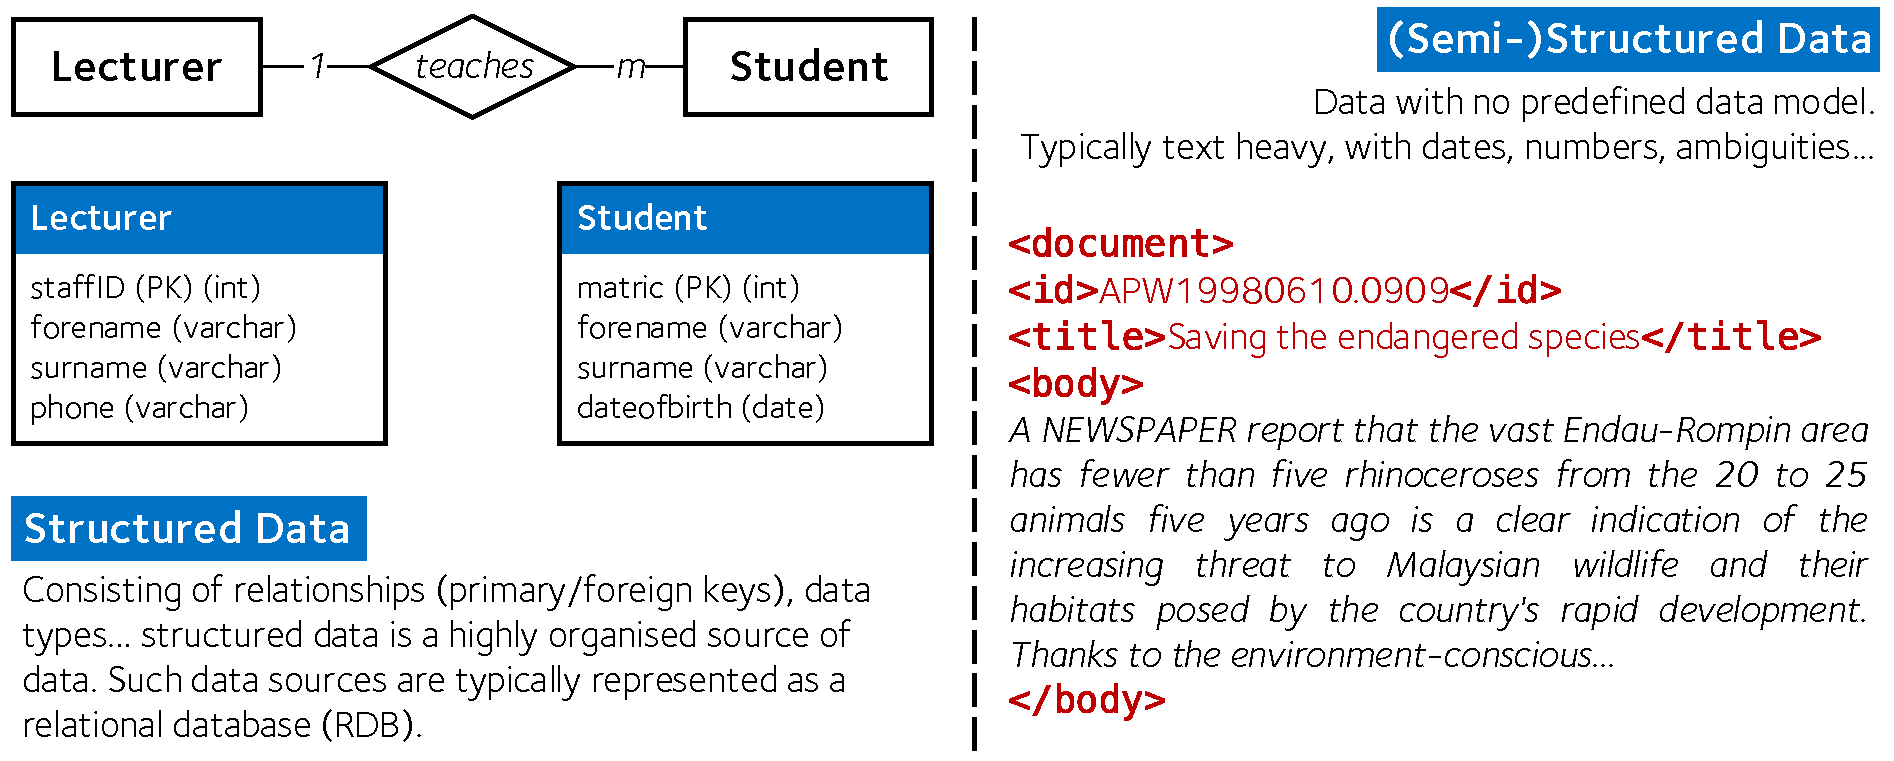
\includegraphics{figures/ch2-structured.pdf}}
    \caption[Structured and (semi-)structured data]{Examples of structured and (semi-)structured data. On the left is a structured~\gls{acr:rdbms} schema, represented in compressed Chen notation. Different types can be specified for each field, representing data in a structured way. On the right, semi-structured data, using a document from the \emph{TREC AQUAINT} newswire collection. Note the semi-structured component at the top of the document (containing an identifier and title), and the unstructured body text.}
    \label{fig:structured_data}
\end{figure}

To complement this challenge, a contemporary~\gls{acr:ir} system is also expected by its users to return results that can be considered \emph{useful} to addressing the searcher's information need, as hypothesised by~\cite{luhn1957ranking_query}, and succinctly expressed by~\cite{robertson1977prp}.

\begin{quote}
    ``A [reference] retrieval system should rank references in the collection in order of their probability of relevance to the request, or of usefulness to the user, or of satisfying the user.''
    \attrib{\cite{robertson1977prp}}
\end{quote}

\blueboxheader{Queries and Results}
A searcher's information need is represented as a \emph{query}. which is in turn comprised of one or more salient \emph{query terms}. The process of converting an information need to a query is known as \emph{query formulation}~\citep{hiemstra2009ir_models}. Depending upon the search domain, the query language used may be artificial. For example, reserved keywords may be utilised to express a \emph{boolean query} (e.g. use of \texttt{AND} or \texttt{NOT} preceding terms -- refer to Section~\ref{sec:ir_background:basics:models:boolean} for more information). Natural language however is considered to be the preferred choice within an~\gls{acr:ir} context~\citep{rijsbergen1979ir}. Given the claim by~\cite{robertson1977prp} above, an~\gls{acr:ir} system then typically returns a series of documents. Depending upon the type of system used, these results my be ranked in order of decreasing perceived relevance by some form of \emph{retrieval model}. The presentation of these results are perhaps known best as the \emph{ten blue links}~\citep{hearst2009_search}, a name given to the way in which web search engines traditionally present results to searchers. If none of the results returned to the searcher can be considered useful in any way to addressing his or her information need, the underlying~\gls{acr:ir} system is largely considered to have failed the searcher~\citep{rijsbergen1979ir}.

\blueboxheader{Operational and Experimental Systems}
\cite{rijsbergen1979ir} defines a difference between \emph{operational} and \emph{experimental}~\gls{acr:ir} systems. While a majority of individuals will only ever interact with an operational, probably commercial~\gls{acr:ir} system (e.g. Google), the work described in this thesis considers purely experimental systems. In order for one to determine how well a particular experimental~\gls{acr:ir} system performs compared to others, a rigid scientific methodology must be employed to allow for fair comparisons. As such, the remainder of this chapter discusses the \emph{de facto} approach that is considered for~\gls{acr:ir} experimentation -- from the setup of such an~\gls{acr:ir} system to the ways in which they can be evaluated.

\subsection{The Cranfield Model}\label{sec:ir_background:basics:cranfield}
The methodology behind the majority of contemporary~\gls{acr:ir} research has centred around the concept of the so-called \emph{Cranfield Model}. Devised, unsurprisingly, at Cranfield University in Bedfordshire, England, the model is based upon the \emph{Cranfield II} experiments~\citep{aslib1966factors}. As highlighted by~\cite{borlund2003iir_model}, the experiments revolve around the notion of \emph{test collections}, with the basic components of the experimental setup illustrated in Figure~\ref{fig:ir_cranfield}. Essentially, the concept of test collections is comprised of three main components.

\begin{itemize}
    \item{A collection of \emph{documents} is provided, which is typically converted to an inverted index before experimentation can begin (refer to Section~\ref{sec:ir_background:basics:indexing}).}
    \item{A collection of \emph{topics} provide a means of simulating different information needs -- and with each topic are one or more \emph{queries} that can be issued to an experimental~\gls{acr:ir} system.}
    \item{Finally, a collection of \emph{relevance assessments} are provided as part of the collection.}
\end{itemize}

\begin{figure}[t!]
    \centering
    \resizebox{1\hsize}{!}{
    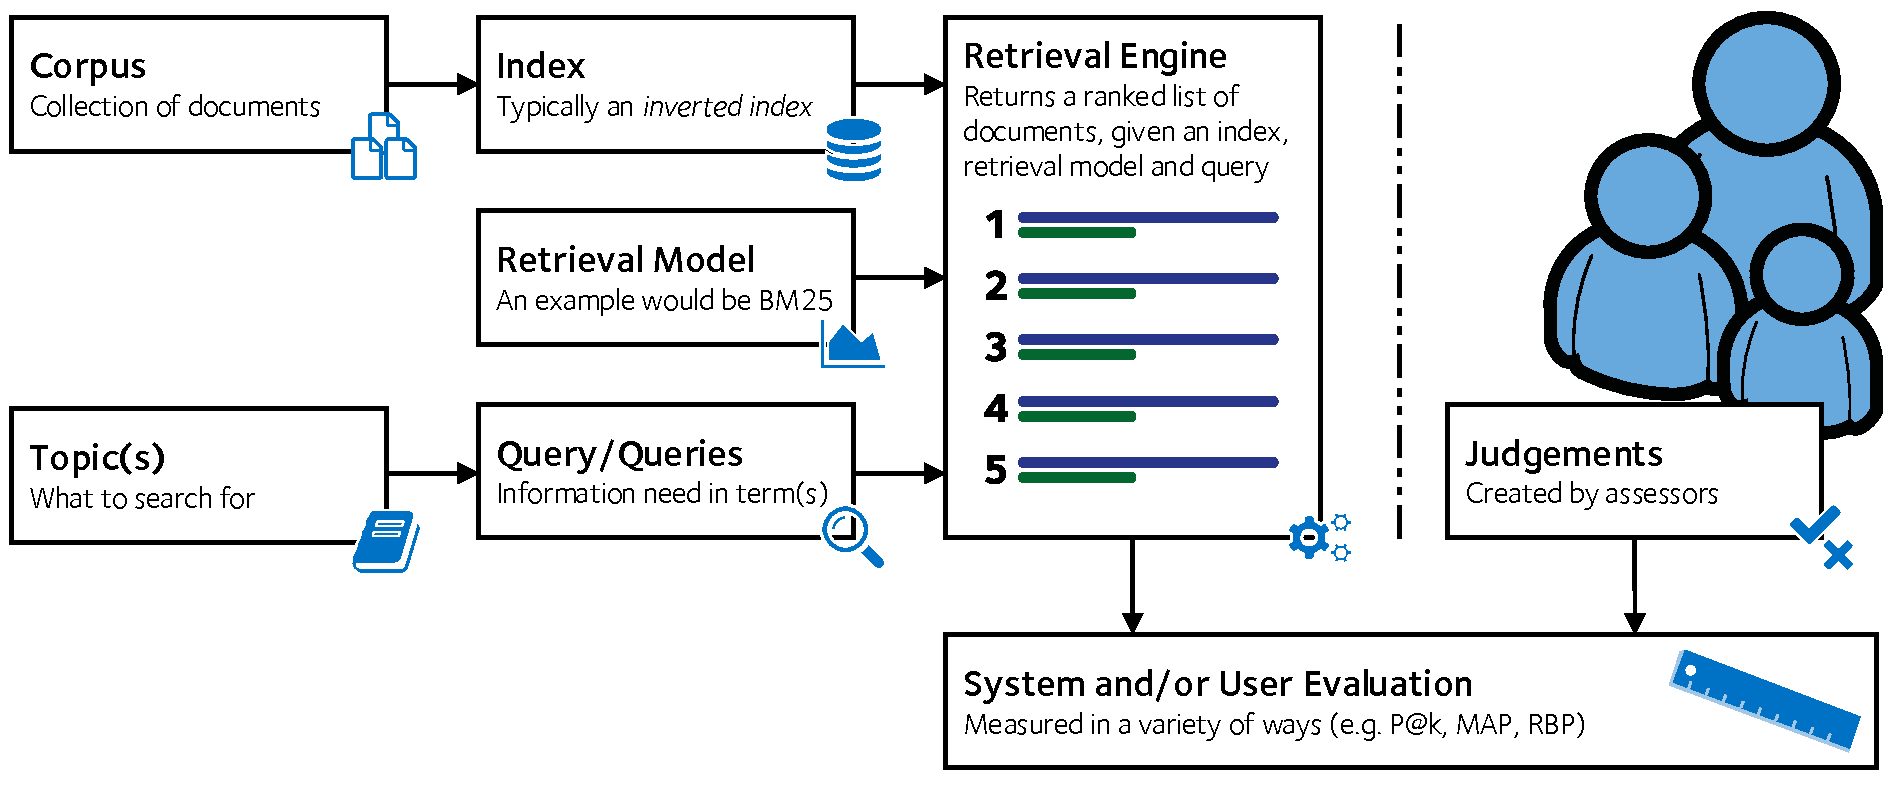
\includegraphics{figures/ch2-cranfield.pdf}}
    \caption[The \emph{Cranfield Model}]{Illustration of the Cranfield Model, the \emph{de facto} approach experimental methodology used for~\gls{acr:ir} research. Given a corpus, topic(s) and document judgements (created by assessors), one can compute various evaluation measures for a given retrieval model and search engine.}
    \label{fig:ir_cranfield}
\end{figure}

In conjunction with the documents and topics, a \emph{retrieval model} is employed (refer to Section~\ref{sec:ir_background:basics:models}), which encapsulates our beliefs about the nature of what constitutes \emph{useful} content. When instantiated, these components are in turn used by the \emph{retrieval engine} to produce a list of potentially useful documents -- called the \emph{matching process}. Many experimental retrieval engines exist, with a non-exhaustive list including: the \emph{Terrier~\gls{acr:ir} platform}\footnote{\url{http://terrier.org/}}; \emph{Apache Lucene}\footnote{\url{https://lucene.apache.org/}}; and \emph{Whoosh}\footnote{\url{https://pypi.python.org/pypi/Whoosh/} -- all URLs mentioned in this footnote were last accessed on March 8\textsuperscript{th}, 2018. \todo{Check they are all on the same page.}}. A specific retrieval engine can be selected based upon the requirements and existing infrastructure available for the particular experiment. In this thesis, for example, we rely upon the Whoosh retrieval engine for all experimental work. Output from the experimental system can then be evaluated using an \emph{evaluation tool} to produce a series of measures to examine the performance of the system (refer to Section~\ref{sec:ir_background:evaluation}).

Relevance assessments are created for each topic of the collection. Assessors examine a series of documents that are extracted from the document collection using a simple query (called \emph{pooling}). For example, given a topic \texttt{wildlife extinction}, a query typically issued to retrieve documents will also be \texttt{wildlife extinction}. The returned documents are then assessed for relevance to the given topic, and a judgement is assigned to each. Typically, such a judgement has been binary, with \texttt{0} denoting non-relevant, and \texttt{1} denoting relevant. The effects of pooling can mean that documents that are potentially relevant can be missed by assessors, and thus will receive no judgement~\citep{keenan2001effect}.

\subsubsection{The Text REtrieval Conference}\label{sec:ir_background:basics:cranfield:trec}
A number of different evaluation forums have been borne out of the Cranfield model. Perhaps most notably is~\gls{acr:trec}, as sponsored by the U.S. Government funded \emph{National Institute for Standards and Technology (NIST)}. Other efforts which have been inspired by~\gls{acr:trec} include \emph{NTCIR}, \emph{CLEF} and \emph{INEX}. Experimentation following the original~\gls{acr:trec} approach is named\emph{~\gls{acr:trec}-style} in this thesis.

Originally organised by Donna Harman and Ellen Voorhees,~\gls{acr:trec} provides a platform for annual collaboration between research groups interested in different aspects of~\gls{acr:ir} research. Each year, a series of~\gls{acr:trec} \emph{tracks} are defined, with each consisting of a collection of documents, topics and relevance judgements. Those who provide the judgements are assessors, usually employees of NIST~\citep{robertson2008history_ir_evaluation}, who were in turn previously employed as news analysts by various U.S. security agencies. Each team wishing to participate in a track receives the collection, and runs them through their experimental search system, following the approach illustrated in Figure~\ref{fig:ir_cranfield}.

Output from the experiments should then be produced in a standardised format. Results can then be used in conjunction with the judgements (termed \emph{Query RELevance judgements}, or \emph{QRELs}), again, as illustrated in Figure~\ref{fig:ir_cranfield}, and fed into a standardised program called \texttt{trec\_eval}\footnote{\texttt{trec\_eval} is downloadable from \url{http://trec.nist.gov/trec_eval/} -- URL last accessed on March 8\textsuperscript{th}, 2018. Version 8.1 of the software was used for computing most of the evaluation measures reported in this thesis.} to perform evaluation of the runs that are undertaken. The application returns the values for a number of common system-sided evaluation measures, some of which are discussed in Section~\ref{sec:ir_background:evaluation}. 

The collaborative (and perhaps competitive) atmosphere that TREC has fostered has broadly been accepted to be good for the~\gls{acr:ir} community. As discussed by~\cite{robertson2008history_ir_evaluation}, some of the main advantages of~\gls{acr:trec} is that it has encouraged a good, formalised scientific methodology for~\gls{acr:ir}. In addition, the provision of providing the community with a large volume of standardised test materials of the quality and quantity in which~\gls{acr:trec} has done is nothing like what was previously available.~\cite{robertson2008history_ir_evaluation} goes on to claim that simply examining the number of research papers published in the field employing some form of~\gls{acr:trec} data is substantial, and that alone is enough to justify the existence of the forum. Standardised sets should also aid reproducibility of research, although we acknowledge that there are other factors at play in order to achieve that goal. 

As previously mentioned,~\gls{acr:trec} is comprised of a series of different tracks, each with its own set of tasks. Some of the tasks, such as those in the \emph{Interactive Track}, as what as known as \emph{ad-hoc}. This type of task can be considered as one of the most obvious for search, when a searcher develops a need for information, and then issues a query to an underlying search engine. Tasks like ad-hoc essentially provide a form of \emph{user model}, one that has been extensively used within~\gls{acr:ir} research for a number of decades. Section~\ref{sec:ir_background:user:models:trec} provides more information on the steps involved in the model, and what it assumes.

\subsection{Indexing Documents}\label{sec:ir_background:basics:indexing}
As previously discussed, the conversion of a series of documents (corpus) into a data structure facilitating fast, full-text search -- as required of an~\gls{acr:ir} system -- is known as \emph{indexing}. This full-text searching is undertaken, usually in milliseconds, in aid of finding useful documents for a given query. Without an index, a retrieval engine would have to manually examine each and every document within a corpus. This would require significant computational power -- and is indeed infeasible for a large scale index, such as the index used in a contemporary commercial web search engine. The additional storage space and management required to maintain an index of documents is considered to be a necessary tradeoff to guarantee timely responses to queries.

\begin{figure}[t!]
    \centering
    \resizebox{1\hsize}{!}{
    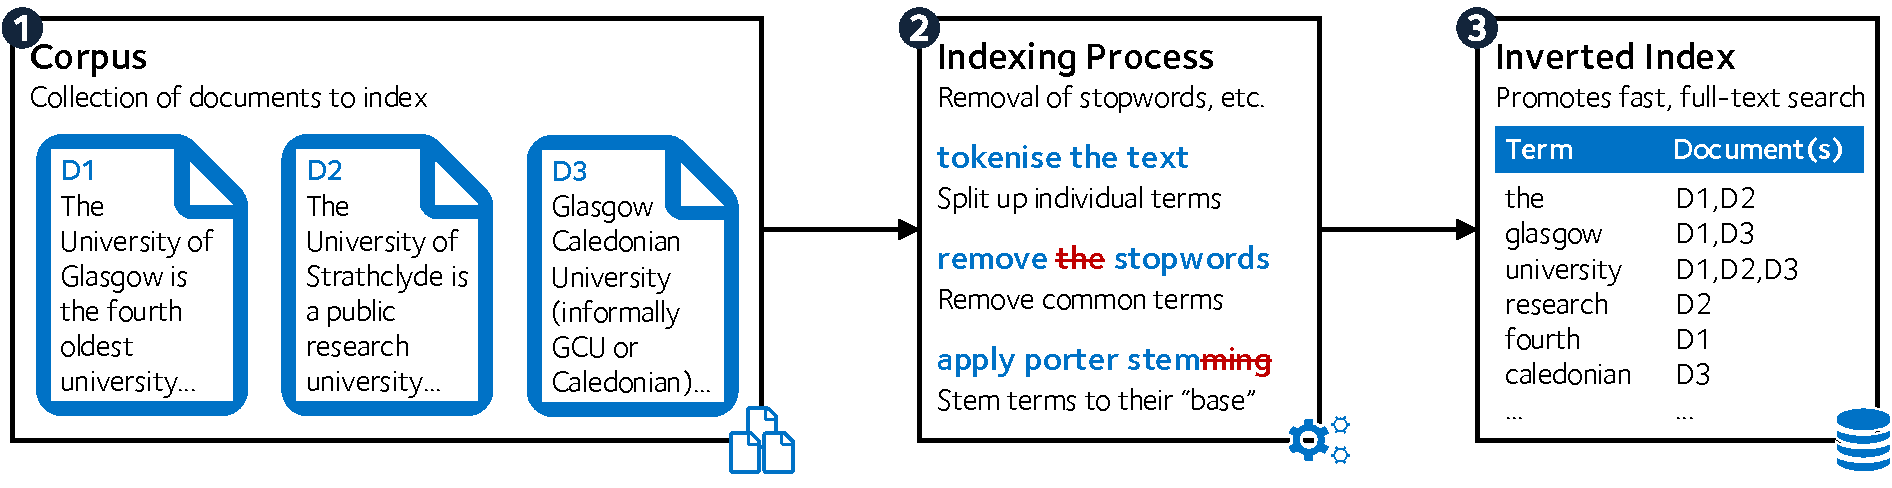
\includegraphics{figures/ch2-inverted.pdf}}
    \caption[Illustration of an \emph{Inverted index}]{A demonstration of an \emph{inverted index}, with three source documents for comparison. Depending upon the requirements of the~\gls{acr:ir} system, the indexing process may vary; all classical~\gls{acr:ir} systems however rely upon some form of inverted index.}
    \label{fig:inverted}
\end{figure}

As illustrated in Figure~\ref{fig:inverted}, the indexing process can be split into three main steps: 

\begin{itemize}
    \item{gathering the corpus of documents to be indexed;}
    \item{performing pre-indexing data preparation; and}
    \item{creating the inverted index.}
\end{itemize}

For the purposes of IR experimentation, most corpora are provided in from the evaluation forum providing the raw materials. As an example, at the time of writing, the University of Glasgow provides the TREC \emph{W2Tg}, \emph{WT10g}, \emph{.GOV} and \emph{.GOV2} document collections.\footnote{Refer to \url{http://ir.dcs.gla.ac.uk/test_collections/} -- URL last accessed March 10\textsuperscript{th}, 2018.}

Running~\gls{acr:ir} experiments with provided test collections is the case for~\gls{acr:ir} experiments following the Cranfield model -- including, of course, TREC experimentation (refer to Section~\ref{sec:ir_background:basics:cranfield:trec}), and the work presented in this thesis. For operational~\gls{acr:ir} systems, data is collated by other means. For example, web search engines employ a \emph{crawler} to examine pages on the~\gls{acr:www} and accumulates more content by following the web's hyperlink structure. Google's crawler for example is called the \emph{Googlebot}, and regularly crawls high impact websites (e.g. popular news sites, such as \emph{BBC News}) to ensure that the associated index is continually refreshed with up to date information. The enormous size of an index that would be employed by Google for web search -- as well as the need for it to be continually updated -- is itself a major engineering challenge, and is not covered in this chapter.

With the indexing process examining each document within the corpora under consideration, a complete \emph{index} will contain an entry for each processed document along with a \emph{vector} of terms that are present within said document. This is known as the \emph{forward index}. An~\gls{acr:ir} system however needs to support fast full-text search, matching terms from a searcher's query to one or more documents within the corpora. To support faster query matching, the most simplistic approach is to \emph{invert} the index, such that the lookup of the index then corresponds to an individual term. A vector of \emph{documents} is then provided for each term, allowing the system much faster access to a potential list of documents. An example of the so-called \emph{inverted index} is provided in Figure~\ref{fig:inverted}. The source corpora in this example illustration contains three documents, and the resultant inverted index is shown. The set of documents retrieved can then be sent to a retrieval model for ranking.

Before a document is indexed however, a number of pre-indexing processes take place on the raw document data as previously mentioned. We now discuss three of the most common processes involved within such a pipeline, including: \emph{tokenisation}, \emph{stopword removal} and \emph{stemming}.

\subsubsection{Tokenisation}
Put simply, tokenisation is the process of \emph{parsing} a source document, and splitting the data within the document into a number of individual \emph{tokens} that may be subsequently indexed. A token is considered a sequence of characters, grouped together to be semantically useful for processing its given document. While we do not go into greater deeper about the process of tokenisation, there are many challenges to this process -- such as \emph{word boundary ambiguity}. While parsing an English or Latin-based document may be relatively straightforward (with spaces representing \emph{word boundaries}), what about other languages, such as Chinese or Japanese? A goal for solving this problem may be to consider what words a potential searcher of an~\gls{acr:ir} system may use to search with in their query.

\subsubsection{Stopword Removal}\label{sec:ir_background:basics:indexing:stopwords}
Stopword removal is another popular choice for indexing document collections for an experimental~\gls{acr:ir} system. Extremely common words which would appear to have little value in selecting documents matching a searcher's query (that is, \emph{non-discriminative} words) can simply be removed from a document's vocabulary entirely. Examples of such words could be \emph{the}, \emph{a}, or \emph{did}. Such words are regarded as \emph{stopwords}. Some experiments consider a small list of stopwords, while others consider a larger list, with larger lists often significantly reducing the size of an indexed corpus~\citep{manning2008ir}. Indeed, it was argued by~\cite{fox1992stopwords} that larger lists ``are advisable''. This was aptly demonstrated by~\cite{dolamic2010stopword}, showing that indexing a with a longer stopword list resulted in significantly improved performance when compared to a much smaller list.

The simplest strategy for producing a list of stopwords would be to count the \emph{term frequency} for each term within a corpus, and sort the list in descending order, selecting some top $k$ of the most frequently occurring terms. Others have produced stopword lists for use in~\gls{acr:ir} research --~\cite{rijsbergen1979ir} produced a list of 250 terms, with~\cite{francis1985stopwords} demonstrating a list of 425 stopwords from the \emph{Brown corpus}\footnote{The \emph{Brown corpus} was a collection of documents representing (then) contemporary American English, compiled by William Francis and Henry Ku\v{c}era -- refer to~\cite{francis1979brown_manual} for more information.}. For the experiments detailed in this thesis, \emph{Fox's classical stopword list}~\citep{fox1992stopwords} is used, consisting of 421 terms. Such an approach may be considered fine, but stopwords lists do vary from collection to collection, as stated by~\cite{lo2005automatically}.

Of course, issues also exist with removing stopwords. For example, what if a searcher issued the query \texttt{to be or not to be}, a phrase from the famous soliloquy of William Shakespeare's \emph{Hamlet?} Such a term could be forgiven to be consisted \emph{entirely} of stopwords. If stopword removal were to be employed, the resultant query to the underlying search engine would contain a grand total of zero terms! As such, commercial search systems are less likely to employ stopword removal~\citep{manning2008ir, dolamic2010stopword} to counter such an issue, employing techniques such as compression to keep the size of the index down. Queries like the one above do contain some meaning -- like tokenisation, there is often more to this problem than meets the eye.

\subsubsection{Stemming}
The final pre-indexing process we consider is \emph{stemming} (also called \emph{lemmatisation}). This is the process of reducing inflected -- or sometimes derived -- words from their \emph{word stem}, \emph{base} or \emph{root}. For example, given the terms \texttt{fisher}, \texttt{fished} and \texttt{fishing}, reducing each of these terms to their respective word stem would result in \texttt{fish}. Essentially, stemming allows one to group words together with a similar, basic meaning. This provides the advantage of reducing the size of an index, and can potentially increase the number of possible matches that can be found with a stemmed set of query terms.

The concept of stemming has been studied since the 1960's, with the \emph{Porter stemmer}~\citep{porter1980algorithm} emerging over time as empirically the most effective.\footnote{The Porter stemming algorithm is not provided in this thesis; refer to~\cite{porter1980algorithm} for an in-depth explanation of the algorithm.} Comprised of a series of linguistic rules, the \emph{measure} of a word can be considered, where \emph{``loosely checking the number of syllables to see whether a word is long enough that it is reasonable to regard the matching portion of a rule as a suffix rather than as part of the stem of the word.''}~\citep{manning2008ir}. Porter stemming is utilised in the indexing process for the work reported in this thesis; other stemmers do exist, such as the original single pass stemmer devised by~\cite{lovins1968development}.

However, issues again exist that must be considered. \emph{Overstemming} is a potential issue, where a word is reduced too far to the point that it loses meaning -- and thus can negatively effect the search results returned. Terms like \texttt{universe}, \texttt{university} and \texttt{universal} when stemmed will be reduced to \texttt{univers}. The three terms are etymologically linked; their modern meanings are however very different. To counter potential issues like this, techniques such as \emph{$n$-grams} may be employed.


\subsection{Retrieval Models}\label{sec:ir_background:basics:models}
In order to achieve the goal of satisfying a searcher's underlying information need, we must have an understanding of how humans comprehend and assess information provided to them. In order to do this, it is argued by~\cite{whiting2015phd} that this requires an intricate knowledge and understanding of the cognitive structures and processes that are responsible for information processing and decision making within the human brain. Much work remains for us to realise this -- our understanding of these processes is limited. Instead,~\gls{acr:ir} researchers have proposed over the decades a series of different mathematically based \emph{retrieval models} that attempt to operationalise the notion of relevance and/or usefulness.

Retrieval models provide us with a means for discussion and further refinement; they provide us with the blueprint from which we operationalise an~\gls{acr:ir} system~\citep{hiemstra2009ir_models}. A retrieval model predicts and explains what a searcher will find, given a query formulated from their underlying information need. The correctness of such a model can then be subsequently tested via experimentation and evaluation. Mathematically defining these key models of an~\gls{acr:ir} system is important as they provide consistency, and ensure that such models can be implemented in the real world.

As previously mentioned, several retrieval models have been defined by different~\gls{acr:ir} researchers over a number of decades, ranging from relatively simplistic to more complex. The more complex approaches not only define a notion of what documents would be considered relevant/useful, but also to what \emph{degree} that is so. This section considers four main retrieval model families in chronological order, with high level summaries of each. We consider: \emph{(i)} the \emph{boolean model}; \emph{(ii)} the \emph{vector space model}; \emph{(iii)} \emph{probabilistic models}; and \emph{(iv)} more recent \emph{language models.} While not totally exhaustive, this broad overview should provide a solid understanding of the developments in developing such models, and the benefits and disadvantages of each approach.


\subsubsection{Boolean Model}\label{sec:ir_background:basics:models:boolean}
Cited as the first formally defined~\gls{acr:ir} retrieval model, the boolean model is also most likely the one to be criticised~\citep{hiemstra2009ir_models}. Introduced originally by~\cite{rijsbergen1979ir}, the model employs operators of mathematic logic as defined by George Boole~\citep{boole1847mathematical} \emph{(set theory)}. Boole defined three basic operators: \texttt{AND}, yielding a logical product between two sets; \texttt{OR}, yielding the logical sum between two sets; and \texttt{NOT}, yielding the logical difference.

\begin{figure}[t!]
    \centering
    \resizebox{1\hsize}{!}{
    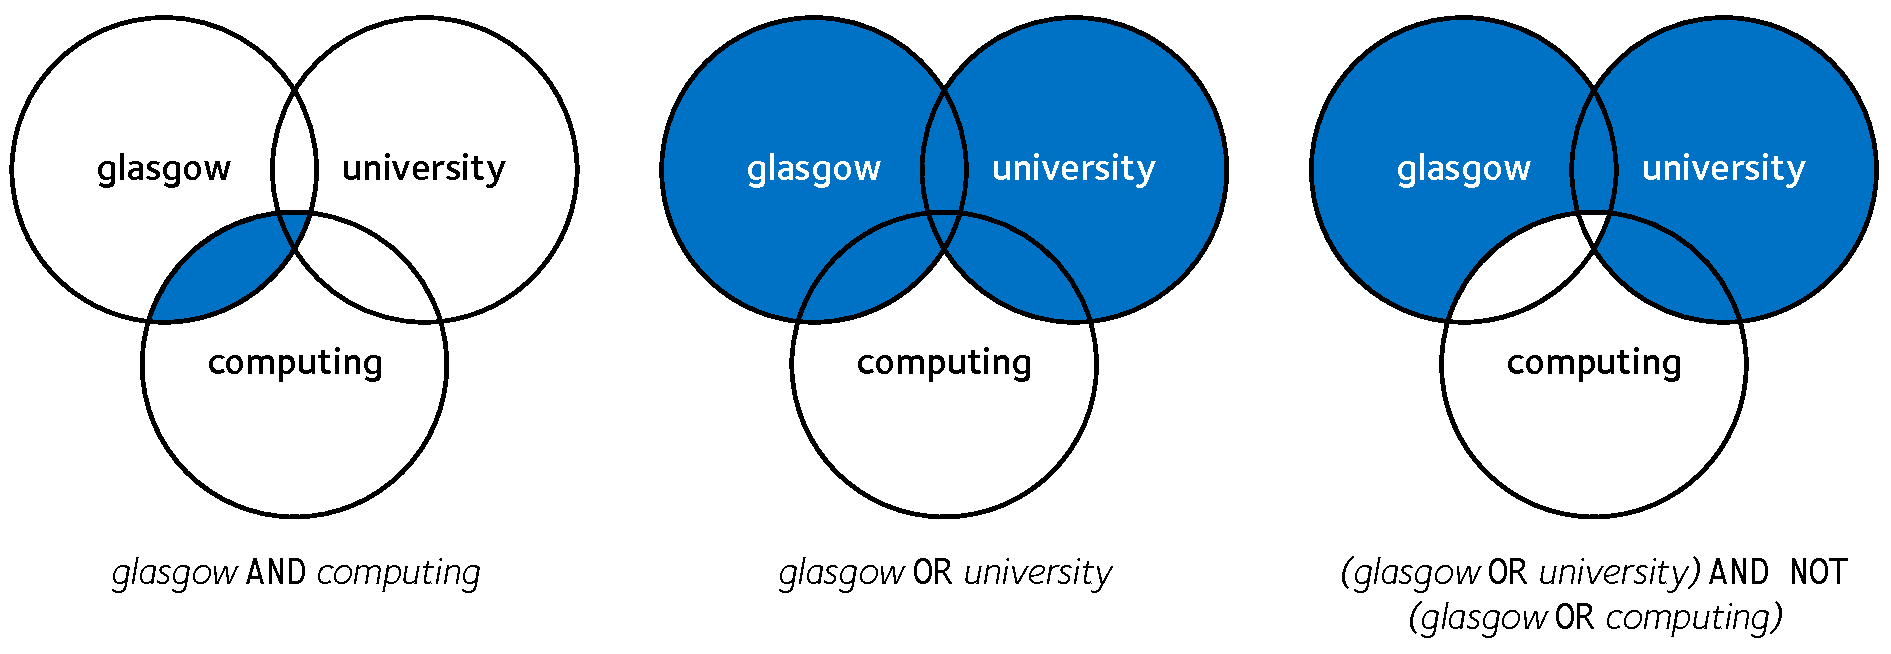
\includegraphics{figures/ch2-boolean.pdf}}
    \caption[Venn diagrams illustrating boolean retrieval]{An example illustration of the boolean retrieval model, using the query terms \texttt{glasgow}, \texttt{university} and \texttt{computing}. Each disc represents the set of documents containing that particular term. In the figure, three Venn diagram examples are provided, demonstrating the key logical operators used (\texttt{AND}, \texttt{OR} and \texttt{NOT}). Areas in blue are returned in the example boolean query provided underneath each Venn diagram.}
    \label{fig:boolean}
\end{figure}

By considering an individual query term as an unambiguous set of documents, logical operations can be applied to retrieve a set of documents. For example, the query term \texttt{glasgow} will yield a set of all documents containing the term \texttt{glasgow}, yet the query \texttt{NOT glasgow} will retrieve the set of documents that \emph{does not} contain any mention of the term \texttt{glasgow}. The results of applying logical operators between different sets can be illustrated through a Venn diagram, where each set of documents is represented as a disc. Figure~\ref{fig:boolean} provides an example of such diagrams.

Despite the relative simplicity of this approach, there are major limitations. First, when considering the query, there is no notion of term importance -- every term has equal weighting. Queries utilising logic rules also appear to be relatively unnatural representations of an information need. Indeed, as the information need become more complex, the boolean query can grow to be disproportionally large and cumbersome to interpret (refer to the right Venn diagram of Figure~\ref{fig:boolean}). This would be especially true when a complex information need is represented as a boolean query. As documents either belong to a set or they don't, a document is either useful (\texttt{TRUE}) or not (\texttt{FALSE}). As such, one cannot estimate a degree to how relevant a document would be to the searcher's query, and thus results are provided to the searcher unranked.

Returning an unranked set of documents would appear as an alien concept to users of~\gls{acr:ir} systems today -- one would assume that the document presented first would be the document considered most likely to be useful as per the underlying retrieval model. This would make it difficult for a searcher to obtain some notion of how many results he or she should examine before stopping, as all terms and documents are considered equal. Despite not being required in contemporary~\gls{acr:ir} systems, many do still provide support for crafting a boolean query for when returning a good set of results is difficult. This may for example be useful when there is ambiguity in the searcher's information need, and clarification is required to eliminate a set of unhelpful documents. Boolean queries also find traction in patent searching, where \emph{recall} rather than \emph{precision} is preferred (refer to Section~\ref{sec:ir_background:evaluation}).

\subsubsection{Vector Space Model}
With major weaknesses present in the boolean retrieval model, work then progressed to develop more advanced approaches that mitigated the issues raised above.~\cite{luhn1957ranking_query} hypothesised that a searcher, when wishing to search for documents addressing their information need, should prepare a document that is similar to the documents that were sought after. By comparing documents against this \emph{representative} document, a system could begin to deduce what other documents would be useful, and by what margin.

The vector space model proposed by~\cite{salton1975vsm} incorporates the principles as outlined by~\cite{luhn1957ranking_query}. These basic principles are operationalised by representing queries and documents within Euclidean geometry, where both are represented as vectors in multi-dimensional space. The notion of how close documents appear to each other denotes the usefulness of a document.

The vector space model is popular, as it provides an intuitive means for addressing the overarching problem of an~\gls{acr:ir} system, and can incorporate methods such as term weighting which have been shown to improve retrieval effectiveness~\citep{croft2010search}. Furthermore, as queries and terms are represented in Euclidean space, vector similarity methods can be employed to determine relevance/usefulness. While many approaches have been trialled, empirical evidence has favoured \emph{cosine similarity}~\citep{croft2010search}. This is aptly illustrated in Figure~\ref{fig:vector_space}. Using such an approach allows one to then compute the degrees of relevance/usefulness, meaning that matched documents can be returned in a ranked order. This ranking than then be potentially utilised by a searcher to determine a cutoff point at which he or she should stop examining results.

\begin{wrapfigure}[13]{r}{0.45\textwidth}
    \begin{center}
    \vspace*{-10mm}
    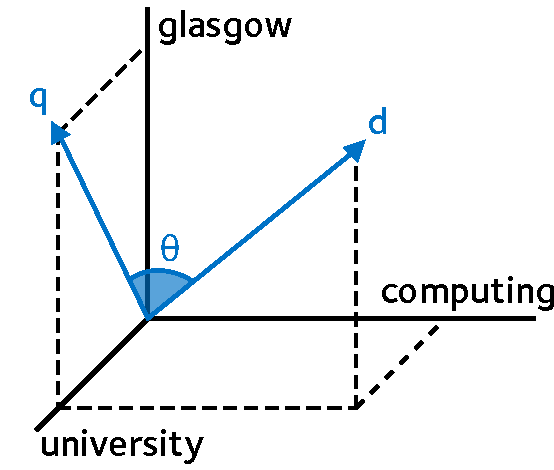
\includegraphics[width=1\textwidth]{figures/ch2-vector.pdf}
    \end{center}
    \vspace*{-4mm}
    \caption[Vector Space Model (Cosine similarity)]{An illustration of the Vector Space Model in Euclidean space, with each term representing a dimension. Here, the cosine similarity between query \emph{q} and document \emph{d} is shown.}
    \label{fig:vector_space}
\end{wrapfigure}

In order to understand the basic workings of the vector space approach, let us consider a query, $Q$, with each of its constituent terms placed within a term vector in $t$-dimensional space, leading to $Q = (q_1, q_2, q_3,\dotsc, q_{it})$. Consider also a document, $D_i$, with terms from the document again represented in $t$-dimensional space, yielding $D_i = (d_{i1}, d_{i2}, d_{i3},\dotsc, d_{it})$. From this notation, $d_{ij}$ represents the \emph{term frequency (TF)} of term $j$ appearing in document $i$. With each term represented as a separate dimension within Euclidean space, a weighting scheme can be subsequently applied to emphasise or understate more discriminative or less discriminative terms, respectively. An example of less discriminative terms would for example be stopwords, as described in Section~\ref{sec:ir_background:basics:indexing:stopwords}. By applying weighting schemes, the vector space model at a stroke overcomes a previously discussed limitation of the boolean model in that all terms are weighted equally.

Term frequency is one of many different term weighting schemes that have been trialled over the years in~\gls{acr:ir} research. Perhaps one of the best and widely used schemes is \emph{inverse document frequency (IDF)}, proposed by~\cite{sparck1972statistical}. Here, the frequency of a term is normalised against the length of a given document. In the words of its creator, IDF allows for one to define the specificity of a term as \emph{``an inverse function of the number of documents in which it occurs.''}~\citep{sparck1972statistical}. This is useful as non-discriminative terms that occur frequently within an index (e.g. \texttt{the}) would have its weight diminished, with the inverse happening for more discriminative terms, better able to describe a given document.

TF and IDF are typically combined together as a measure of both term appearance and importance, under an approach called \emph{TF-IDF}. For a given term $k$, one can calculate a TF-IDF score with the following equation.

\begin{equation*}
tf_{i,k} \cdot idf_{k} = \frac{f_{i,k}}{\sum_{j=1}^{t} f_{i,j}} \cdot log \frac{N}{n_k}
\end{equation*}

Above, $f_{i,k}$ is the frequency of term $k$, $N$ is the number of documents in the collection used, and $n_k$ is the number of documents in which term $k$ appears at least once.

\subsubsection{Probabilistic Models}
From boolean to vector space retrieval models, a further model emerged based upon \emph{probability theory}. Probability theory allows one to define a means to formally model the relevance and/or usefulness of a document to a searcher's query, given \emph{uncertainty} about their precise information need. One of the most widely referred to ranking principles, known as the \emph{Probability Ranking Principle (PRP)} (defined by~\cite{robertson1977prp} -- who in turn attributed the development to~\cite{cooper1971relevance}), states the following.

\begin{quote}
\emph{``If a reference retrieval system's response to each request is ranking of the documents in the collections in order of decreasing probability of usefulness to the user who submitted the request, where the probabilities are estimated as accurately as possible on the basis of whatever data has been made available to the system for this purpose, then the overall effectiveness of the system to its users will be the best that is obtainable on the basis of that data.''}
\attrib{\cite{robertson1977prp}}
\end{quote}

Essentially, this states that documents that are considered more likely to be relevant than non-relevant should be retrieved -- or where $P(R|D) < P(\overline{R}|D)$. However, while the PRP lays much of the foundation from which probabilistic retrieval models have been derived, it does not itself provide a concrete implementation of such a model. The framework provided by the PRP in order to score a document to a searcher's query is:

\begin{equation*}
score(d,q) = P(rel|q,d) \approx \sum_{t \in q}wt_{t,d}.
\end{equation*}

Above, $rel$ is defined as the relevance probability of document $d$, given query $q$. Early approaches following this framework utilised Bayes' theorem to define the probability of a document being relevant to the associated query, based upon the likelihood of drawing query terms from relevant and non-relevant documents. This was considered as a classification problem, where documents were considered as either relevant or non-relevant to said query. The aforementioned likelihood has been computed by many models -- perhaps the most important being \emph{Okapi BM25}~\citep{robertson1995trec3}. Indeed, this retrieval model has had considerable impact upon the~\gls{acr:ir} community and is still used extensively today, providing a solid baseline for contemporary research. This model is employed as the basic retrieval model for experimentation in this thesis due to its effectiveness and popularity.

\subsubsection{Language Models}
The final retrieval model family that we discuss are language models, closely related to the probabilistic model we define above. Indeed, while such probabilistic models have been demonstrated to perform well empirically, adapting the PRP and subsequent developments to more advanced approaches has been difficult and is generally not intuitive~\citep{hiemstra2000language_modelling} -- the interpretation offered by probabilistic models may be considered loose, and is not always theoretically principled~\citep{whiting2015phd}. This has led to the development of more formalised statistical language modelling approaches, as defined in the fields of \emph{Natural Language Processing (NLP)}, for example~\citep{lavrenko2001language_models}.

Given the strong rooting in the principles of language and associated fields, language models provide a solution to the so-called \emph{bag of words}~\citep{harris1954distributional} concept that a majority of preceding retrieval models subscribe to. Put simply, this concept considers each document and query as a bag of words, meaning that the ordering of terms loses any significance. While a simplifying assumption, losing the ordering of terms means that semantic meaning and grammar rules are lost -- and thus a retrieval engine employing a model using this simplifying assumption may lose key meanings, and subsequently retrieval effectiveness will suffer.

Essentially, a language model is a probability distribution over strings of text. Given a string of text (i.e. a searcher's query), how likely is it that the given query appears in a given \emph{language}? Each document provides its own language, where we consider all possible phrases that the author of a document could have written when creating said document. Of course, some phrases are more likely than others. For example, the phrase \texttt{rain in glasgow} is more likely to appear in a document (in that order) than the seemingly random assortment of terms \texttt{purple monkey dishwasher}\footnote{If you ever watched \emph{The Simpsons}, you might disagree with this statement.}. Given this, and conceptualising a searcher's query in much the same fashion, we can produce a probability distribution $P(Q|D)$, concerning the probability of observing query $Q$ during some form of sampling within the language model of document $D$.

The most simplistic approach to language modelling is undoubtedly the \emph{unigram} approach, where each term within a document and/or query are considered in isolation, which subscribes to the aforementioned simplifying bag of words concept. Essentially, such an approach provides a probability distribution over the words appearing in the language. Higher order \emph{grams} such as \emph{bi-grams} and \emph{tri-grams} begin to consider more the place in which terms appear with respect to others, and thus the semantic meaning defined by this positioning begins to be taken into account within the probability distribution. When considering a document, the more a document discusses a particular topic, the more likely one would begin to observe terms about that topic in said document. When a term is not mentioned in a document, smoothing can be applied (given the wider collection the document is part of) to avoid a zero probability when calculating the probability of terms permitting the partial matching of queries where not all terms appear within a target document.

\subsection{Evaluating Systems}\label{sec:ir_background:evaluation}
Given the \emph{de facto} architecture of an experimental~\gls{acr:ir} system (Section~\ref{sec:ir_background:basics:cranfield}) and the numerous retrieval models that one can employ (Section~\ref{sec:ir_background:basics:models}), how can we then begin to evaluate a given retrieval system? Recalling that the \emph{modus operandi} of such a system is to satisfy the needs of the searchers who utilise it,~\cite{lancaster1968information} provides three criteria by which an~\gls{acr:ir} system can be evaluated:

\begin{itemize}
    \item[\emph{(i)}]{the suitability of an~\gls{acr:ir} system in terms of the specific tasks for which it will be used;}
    \item[\emph{(ii)}]{the~\gls{acr:ir} system's task performance \emph{efficiency}; and}
    \item[\emph{(iii)}]{the extent to which the system satisfies the information needs of its \emph{users.}}
\end{itemize}

These three criteria can themselves be subsequently split into two separate categories: approaches that consider how well the \emph{system} performs (i.e. criterion \emph{(i)} and \emph{(ii)}); and with regards to the individual who is using the~\gls{acr:ir} system at the time (\emph{user-orientated}, criterion \emph{(iii)})~\citep{voorhees2005trec_book}. Given the title of this section, we subsequently only consider system-orientated evaluation approaches here; a more detailed explanation of a user's role and how we can evaluate their performance is provided in Section~\ref{sec:ir_background:user:evaluation}.

Considering system-orientated measures of evaluation, one can consider a system's \emph{efficiency} or \emph{effectiveness}. Efficiency concerns some form of operational metric, such as the speed of the~\gls{acr:ir} system. This example is important (especially in commercial web search engines) as even a fractional increase of the time taken to return results to a searcher can reduce the number of returning searchers, and impacts search engine revenue~\citep{brutlag2009speed}. Indeed, this is examined in more detail in Chapter~\ref{chap:temporal}.

However, when one thinks of~\gls{acr:ir} evaluation, they usually think about how \emph{effective} the system is. Of course, the definition of what defines an~\gls{acr:ir} system to be effective hugely depends upon the type of search task being undertaken. A patent searcher would for example expect an~\gls{acr:ir} system to return \emph{all} relevant patents to avoid missing a related patent (and thus incurring penalties) -- whereas a casual web searcher curious about a topic they know little about (i.e. ad-hoc) would be satisfied with a single, relevant result.

As such, this section provides a brief overview of the basic effectiveness measures widely used within~\gls{acr:ir} today. We consider four different measures.

\begin{figure}[t!]
    \centering
    \resizebox{1\hsize}{!}{
    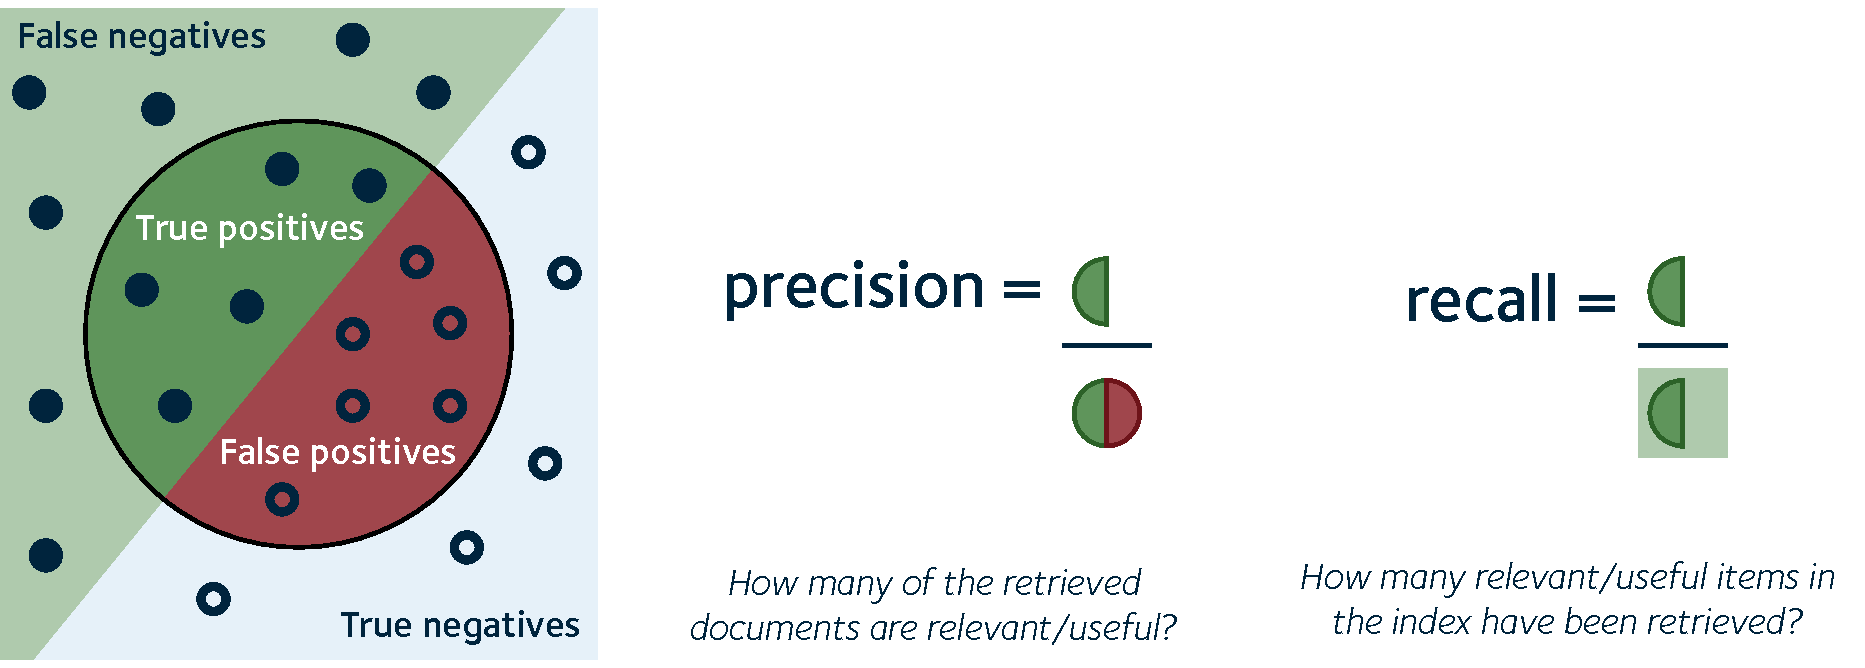
\includegraphics{figures/ch2-pr.pdf}}
    \caption[Precision and recall]{An illustration of precision and recall. On the left is an illustrated example of an index, containing many documents. The large circle represents the set of documents retrieved for a query. Documents that are relevant to the query are represented as~
\includegraphics[height=\fontcharht\font`\d]{figures/ch2-pr-r.pdf}, with non-relevant documents represented as~
\includegraphics[height=\fontcharht\font`\d]{figures/ch2-pr-nr.pdf}. Note that not all relevant documents are retrieved; doing so would mean that the retrieval engine used would have produced perfect results. From the illustration on the left, definitions of \emph{precision} and \emph{recall} are also provided.}
    \label{fig:pr}
\end{figure}

\subsubsection{Precision}
The \emph{precision} ($p$) of an~\gls{acr:ir} system considers the fraction of documents that have been retrieved that are considered to be relevant or useful to the searcher's given query, information need. An~\gls{acr:ir} system that yields high precision is generally regarded as one that performs well.

Figure~\ref{fig:pr} provides a visual illustration of what precision entails (as well as its counterpart, \emph{recall}, which is discussed below). Given the set of all documents within an index, an~\gls{acr:ir} system will retrieve a number of these documents that satisfy the criteria set out in the retrieval model employed. Of the documents retrieved, some will be considered relevant to the searcher's information need; others will be considered non-relevant. As such, prior knowledge of the relevance of particular documents to given topics is therefore required (e.g. TREC QRELs, as defined in Section~\ref{sec:ir_background:basics:cranfield:trec}).

Precision can therefore be defined as:

\begin{equation*}
precision = \frac{|~\text{\emph{relevant documents}}~\cap~\text{\emph{retrieved documents}}~|}{|~\text{\emph{retrieved documents}}~|}.
\end{equation*}

Research in~\gls{acr:ir} typically reports precision up to a particular rank, i.e. $p@k$. For example, $p@10$ will provide a fractional value for the number of relevant documents that appeared within the top $10$ results of a query. Herein lies one of the most elementary and basic \emph{stopping models} that we find encoded within various measures and models defined by~\gls{acr:ir} researchers over the years -- stopping at $10$, or $k$, denotes that a system or searcher need not bother examining any further documents.

\subsubsection{Recall}
While precision considers the fraction of documents retrieved that are relevant, \emph{recall} ($r$) considers the fraction of documents that were retrieved and relevant to a query against \emph{all known relevant documents for a query}. Recall can formally be defined as:

\begin{equation*}
recall = \frac{|~\text{\emph{relevant documents retrieved}}~|}{|~\text{\emph{relevant documents}}~|}
\end{equation*}

Considering the patent searching example defined above, high recall would be desirable in this type of task -- high recall means more patents matching the searcher's query will be returned, thus reducing the possibility of missing important prior filings.

Given more modern retrieval models, the notion of ranking would lead a searcher to assume (as per the PRP~\citep{robertson1977prp}) that relevant documents pertaining to their query will be the first results presented. Non-relevant documents will also of course appear, typically leading to some form of tradeoff between precision and recall, as discussed below. The tradeoff considers the notion that as you increase recall, the number of non-relevant items will undoubtedly also increase, thus reducing the~\gls{acr:ir} system's overall precision.

\subsubsection{F-Measure}
Considering the aforementioned tradeoff between precision and recall, the \emph{F-measure}, which represents a \emph{weighted, harmonic mean} between the two. Originally proposed by~\cite{rijsbergen1979ir}, the measure was provided to \emph{``measure the effectiveness of retrieval with respect to a user who attaches $\beta$ times as much importance to recall as precision.''} The F-measure, along with its $\beta$ parameter, is defined by~\cite{chinchor1992f_measure} as:

\begin{equation*}
F_\beta = \frac{(\beta^2 + 1)\cdot pr}{\beta^2 \cdot p + r}\hspace{10mm}(0\leqslant\beta\leqslant+\infty).
\end{equation*}

Above, $p$ and $r$ denote precision and recall respectively. $\beta$ is simply used as a parameter for controlling the balance between the two. When $\beta = 1$, $F_1$ is equivalent to the harmonic mean of precision and recall. Since the terms F-Measure and harmonic mean are ubiquitously linked (somewhat \emph{harmoniously}\dots), the two terms are used interchangeably within the literature. As $\beta$ tends towards $0$, the score becomes more precision orientated.

\begin{figure}[t!]
    \centering
    \resizebox{1\hsize}{!}{
    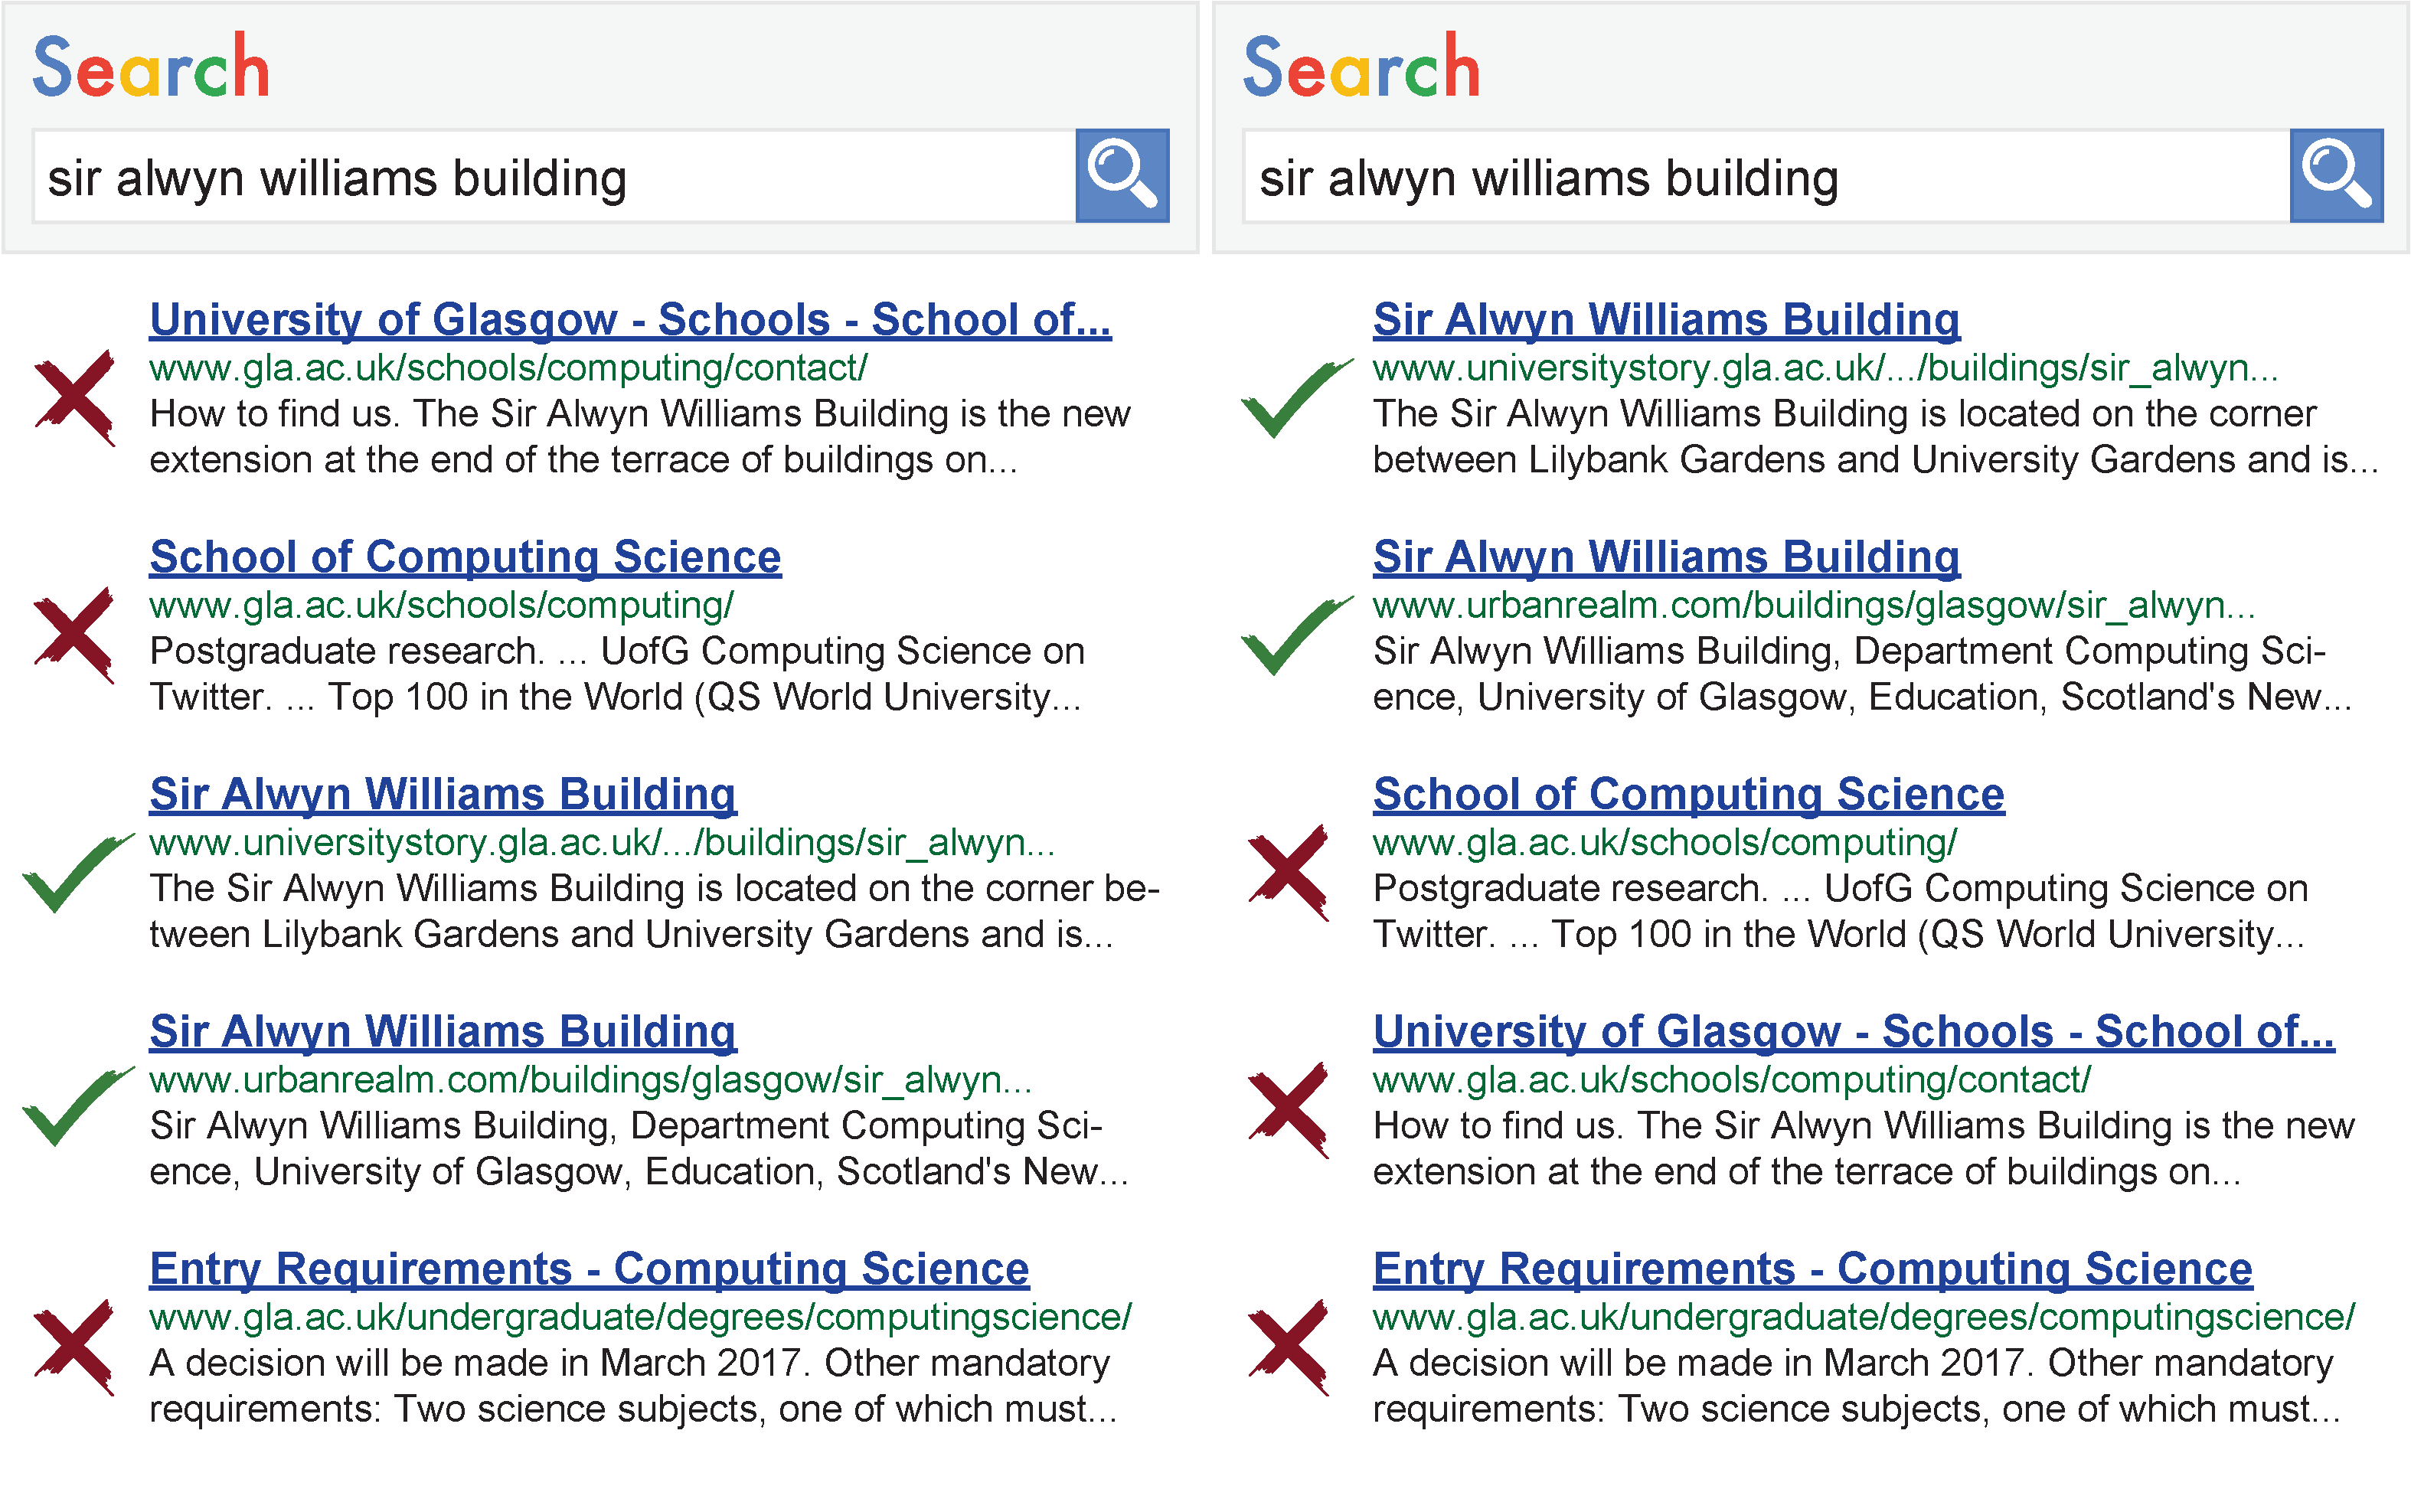
\includegraphics{figures/ch2-ranking.pdf}}
    \caption[The importance of ranking]{Given an information need to find out information about the \emph{Sir Alwyn Williams Building} (part of the University of Glasgow's estate portfolio), which ranked list of results would you prefer to make use of?}
    \label{fig:ranking}
\end{figure}

\subsubsection{Mean Average Precision}
One of the major limitations of the previously examined measures is that the \emph{ranking} of results is not specifically taken into consideration. For example, consider Figure~\ref{fig:ranking}. Looking at the {\color{dmax_green}ticks} and {\color{dmax_red}crosses} (denoting relevant and non-relevant content, respectively) within the figure, would it be desirable to be presented with the list of results ranked in order shown on the left, or on the right? Despite apparent differences in the ranking of results, precision for example would show no difference -- both ranked lists contain two relevant documents, and three non-relevant. A simple calculation would show that the $p@5$ score for both lists would therefore be $2 / 5 = 0.4$ -- there is no discernible difference between them.

One of the most widely used measures that addresses this issue -- and provides a means of quantifying the all-round effectiveness of a retrieval system for a representative set of test topics -- is \emph{Mean Average Precision (MAP)}~\cite{voorhees2005trec_book}. Rather than considering a single set of results, MAP can consider multiple queries -- and, as alluded to above, considers the ranking in which results for each query are provided.

As the name might imply, MAP provides a mean over the \emph{Average Precision (AP)} for each topic that is examined. AP provides the rank sensitive component of MAP up to some cuttoff $k$, as defined below:

\begin{equation*}
AP = \frac{\sum^{n}_{k=1}(p(k) \cdot rel(k))}{|~\text{\emph{relevant documents}}~|}.
\end{equation*}

Above, $P(K)$ is the precision cutoff at rank $k$, and $rel(k)$ is a function to denote the relevance of a particular document at rank $k$. This is assumed to be binary, with $1$ denoting a relevant document, and $0$ denoting a non-relevant document. The AP is then computed for each sample query, $q$, over the set of topics $T$ to produce a final MAP score for the~\gls{acr:ir} system:

\begin{equation*}
MAP = \frac{\sum^{T}_{q=1} AP(q)}{|~Q~|}.
\end{equation*}


\section{Considering the User}\label{sec:ir_background:user}
central to all of this is the user.
talk about diane's spectrum of IR experimentation, from system to user focused.
consider a variety of more user-centric evaluation approaches.
here, you can also bring in the notion of simulation
mention that this is IIR.

\begin{figure}[t!]
    \centering
    \resizebox{1\hsize}{!}{
    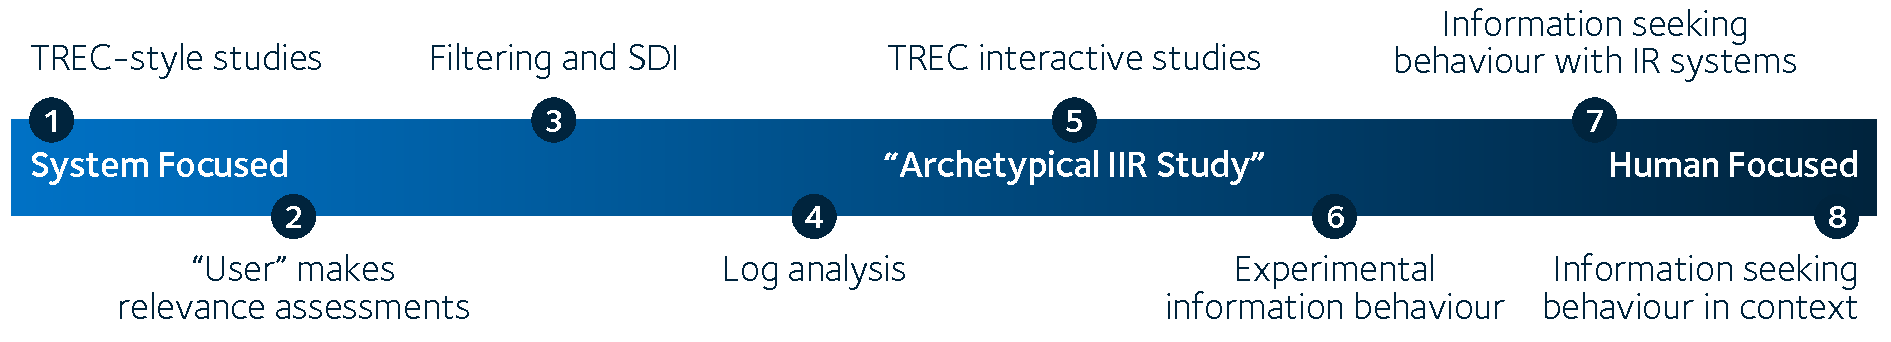
\includegraphics{figures/ch2-spectrum.pdf}}
    \caption[The spectrum of conceptualising IIR research~\citep{kelly2009iir}]{The spectrum of conceptualising IIR research. Methods on the left consider a more system-focused approach, with those on the right considering a more user-focused approach. The fifth step within the spectrum considering TREC interactive studies is considered to be an \emph{"archetypical~\gls{acr:iir} study"}. Figure adapted, with permission, from~\cite{kelly2009iir}.}
    \label{fig:spectrum}
\end{figure}

\subsection{Simulating the User}\label{sec:ir_background:user:simulation}

\subsection{Considering User Models}\label{sec:ir_background:user:models}

\subsection{Evaluating User Performance}\label{sec:ir_background:user:evaluation}

\subsubsection{Relative Relevance}
~\cite{borlund1997iir_evaluation}

\subsubsection{Ranked Half-Life}
~\cite{borlund1997iir_evaluation}

\subsubsection{Cumulative Gain}

\subsubsection{Rank-Biased Precision}

\subsubsection{INST}

\section{User Models}

\subsection{The TREC-Style User}\label{sec:ir_background:user:models:trec}




    - diane kelly's spectrum of system to user orientated
        - TREC/Cranfield is a very basic approach to simulation
            a model of how user performs
        - user orientated approach looks at how users interact with the system
        - models of how users search... to show how we develop models.
        
        - at the end of chapter

Look at Kelly (2009) -- Methods for Evaluating Interactive Information Retrieval Systems with Users

these measures/evaluations are thining about the way people go and search
of relevance to this thesis are stopping strats
diff. measures encoe different stopping models. different ways of evaluating this.
in the next chapter, provide an overview of the different types of models of search, and how searching has been conceptualised with respect to stopping strategies.

\subsection{Towards User-Orientated Measures}

Stephen Robertson has good points in his paper on IR evaluation history:~\cite{robertson2008history_ir_evaluation}

Cranfield isn't very good. Furthermore, this model uses only binary and topical-oriented relevance. The conclusion is that the batch-driven mode of the Cranfield model is not suitable for the evaluation of IIR systems, which, if carried out as realistically as possible, requires human interaction, potentially dynamic information need interpretations, and the assignment of multidimensional and dynamic relevance. (From Borlund 2003)


\subsection{TREC Ad-Hoc}\label{sec:ir_background:user:trec}
\todo{does this bit need to be moved to the next chapter?}
- searcher acquires an information need, sits down, and conducts a search against an existing collection of documents over a set period of time. Known as ad-hoc retrieval, or retrospective searching in older literature.

- this is lifted from Robertson (2008), rephrasing required, and probably needs to be moved to the user model part.

- The user model invoked here is what has now become the most obvious one for search: user has an
information need, sits down in front of a system and conducts a search against an existing collection of
documents, over a limited time period. This is known in TREC jargon as an ‘ad-hoc’ search – an earlier more-orless
equivalent term was ‘retrospective searching’. System produces a ranked list of items, which the user consults
in rank order. Users may judge documents good or bad, but in principle there may be any number of good
documents in the collection. (The one significant change in this model from the Cranfield view is that there is now
an assumption that each system will rank its results list.) It is often asserted that there is also an assumption that
requests are topical or subject-based (documents about X); indeed the TREC jargon, which is to call requests
‘topics’, encourages that view18. However, although most of the requests used in TREC (all of those in early
TRECs) are indeed topical, there is no necessary requirement of the model that this should be so, or that they
should be purely topical. In some sense the nature of the requests is determined by the relevance judgements; if
the judgements depend on other criteria than pure topicality, then that is the nature of the task.
However, it is fundamental to the model that the judge or assessor should indeed be able to make a judgement
on each document, actually a binary one for most of the TREC ad-hoc tasks, and should be able to make the
judgement irrespective of the order of presentation of the documents. This last precludes, for example, embedding
a criterion of novelty in the usual ad-hoc task relevance judgements (although one track did investigate novelty by
making judgements of novelty separated from the relevance judgements). A typical TREC ‘topic’ has a short title (which might be used directly as a query), and additional information about the
supposed information need under the headings ‘description’ and ‘narrative’. The narrative contains explicit rules for
judging the relevance of documents. An example title and description are: Hydroponics—Document will discuss the
science of growing plants in water or some substance other than soil. 


\section{Chapter Summary}



Basic concepts -- given a query, tries to satisfy that query.
Follows a system-orientated methodology

From Leif:
- indexing
    tokenizers, etc
- retrieval models
    - these models have some notion of how much someone should retrieve/stop.
    - boolean, look at whole set of documents
    - other models, there's a cutoff... e.g. cosine similarity, angle gets too large, so you stop.
    - probabilistic ranking principle
    
        \begin{quote}
            ``If a reference retrieval system's response to each request is a ranking of the documents in the collections in order of decreasing probability of usefulness to the user who submitted the request, where the probabilities are estimated as accurately as possible on the basis of whatever data has been made available to the system for this purpose, then the overall effectiveness of the system to its users will be the best that is obtainable on the basis of that data.''
            \attrib{W.S. Cooper, in private correspondence to~\cite{robertson1977prp}.}
        \end{quote}
    
    
        - decreasing probbaility of relevance
        - get odds of rel over non-rels, so there is some idea of a cut-off.
        - why would you look at a document that is less relevant?
        - nobody uses it, just make this observation.
- evaluation
    - effects of pooling in judgements?
    - system orientated (cranfield)
        - precision
        - recall
    - user orientated
    
    - diane kelly's spectrum of system to user orientated
        - TREC/Cranfield is a very basic approach to simulation
            a model of how user performs
        - user orientated approach looks at how users interact with the system
        - models of how users search... to show how we develop models.
        
        - at the end of chapter

% \subsection{Methodologies}
%
% \subsubsection{System-Orientated}
%
% \subsubsection{User-Orientated}
%
% \subsection{Retrieval Models}
%
% \subsubsection{Boolean Model}
%
% \subsubsection{Vector Space Model}
%
% \subsubsection{Probabilistic Models}
%
% \subsubsection{Language Models}
%
% \subsection{Search Tasks}
%
% \section{Evaluating Retrieval Effectiveness}\label{sec:ir_background:evaluation}
% Basic measures and models.
%
% \subsection{Precision}
%
% \subsection{Recall}
%
% \subsection{Mean Average Precision}
%
% \subsection{F-Measure}
%
% \subsection{Towards User-Orientated Measures}
%
% \subsection{User Models}
% these measures/evaluations are thining about the way people go and search
% of relevance to this thesis are stopping strats
% diff. measures encoe different stopping models. different ways of evaluating this.
% in the next chapter, provide an overview of the different types of models of search, and how searching has been conceptualised with respect to stopping strategies.